\chapter{Quantum Fourier Transform}
\section{Fourier Transform}
The Fourier Transform of a discrete set of numbers $x_0,x_1 ... x_{N-1}$ is defined as the set of numbers $y_0,y_1....y_{N-1}$ where :
\begin{equation}
y_k = \frac{1}{\sqrt{N}} \sum_{j=0}^{N-1} x_j e^{2 \pi ijk/N }
\end{equation}where $i = \sqrt{-1}$. Like any other transformation, Fourier transform also has an inverse:
\begin{equation}
FT^{-1}(\{y_0,y_1...y_{N-1}\}) = \{x_0,x_1,...x_{N-1}\} \text{ where } x_k = \frac{1}{\sqrt{N}} \sum_{j=0}^{N-1} y_j e^{-2 \pi ijk/N }
\end{equation}
In case of quantum systems, Fourier transform is defined to be the linear operator:
\begin{equation}
\sum_{j=0}^{N-1} x_j|j\rangle \rightarrow \sum_{k=0}^{N-1} y_k|k\rangle
\end{equation}where the sets, $|j\rangle$ and $|k\rangle$, are the basis states and $\{y_0,y_1...y_{N-1}\}$ are the classic Fourier transform of $\{x_0,x_1,...x_{N-1}\}$.\\
Fourier Transform is useful in a variety of fields like signal processing, image processing etc. and hence computing the Fourier Transform is essential. \\
\section{Classical Solution}
In case of classical computers, the best known algorithm for computing Fourier Transform is the Fast Fourier Transform(FFT). The time-complexity of this algorithm is $O(N \log{N})$ where N are the number of elements in the sequence.\\
FFT is the set of algorithms which uses the divide and conquer strategy to compute the Discrete Fourier Transform. The most common of them is the \href{https://en.wikipedia.org/wiki/Cooley-Tukey_FFT_algorithm}{Cooley-Tukey FFT algorithm}. It divides the set of numbers into two sets based on whether they are even or odd. Then, it computes the Fourier Transform $E_k$ and $O_k$ of these smaller sets. Then, the fourier transform of the whole set i given by:
\begin{equation}
\begin{split}
Y_k = E_k + e^{-\frac{2\pi i}{N}k} O_k\\
Y_{k+\frac{N}{2}} = E_k - e^{-\frac{2\pi i}{N}k} O_k
\end{split}
\end{equation}The algorithm can be used to compute the FT on the series of even and odd sets i.e. $E_k$ and $O_k$. Note that the algorithm divides the problem of FT of a series into two problems of computing the FT on sub-series and hence it is a divide and conquer algorithm. The combining step takes $O(n)$ time and hence the Time complexity equation becomes:
\begin{equation}
T(N) = 2T(\frac{N}{2}) + O(N)
\end{equation}By using the Master's Theorem, we get that $T(N) = O(N \log{N})$.
\begin{figure}[h]
\centering
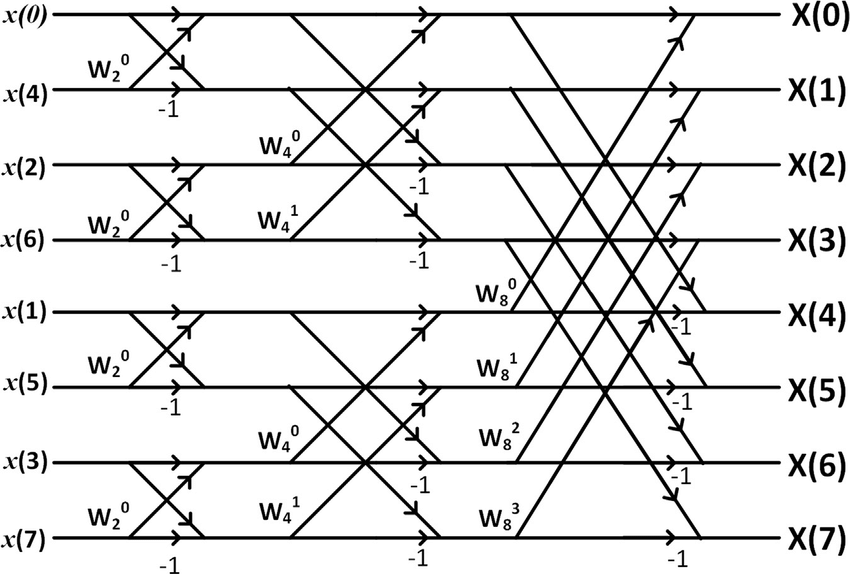
\includegraphics[width=0.5\textwidth]{images/fft.png}
\label{fft}
\caption{Butterfly diagram for the Cookey-Tukey FFT algorithm}
\end{figure}
\section{Quantum Solution}
In the case of Quantum Computing, the complexity to calculate the Quantum FT is $O(n^2)$ where $N = 2^n$, an exponential speed-up as compared to the classical case!! \\
To understand the algorithm used for the QFT computation, we must first re-write the expression for QFT.
\begin{equation}
\begin{split}
QFT_N|x\rangle &= \frac{1}{\sqrt{N}} \sum_{y=0}^{N-1} e^{\frac{2\pi iyx}{N}} |y\rangle
\\ &= \frac{1}{\sqrt{2^n}} \sum_{y=0}^{N-1} e^{\frac{2\pi iyx}{2^n}} |y\rangle
\\ &= \frac{1}{\sqrt{2^n}} \sum_{y=0}^{N-1} e^{2\pi ix\frac{\sum_{k=1}^{n}y_k}{2^k}} |y_1y_2....y_n\rangle \text{ where $(y_1y_2....y_n)$ is the binary representation of y}
\\ &= \frac{1}{\sqrt{2^n}} \sum_{y=0}^{N-1} \prod_{k=1}^{n} e^{2\pi ix\frac{y_k}{2^k}} |y_1y_2....y_n\rangle 
\\ &= \frac{1}{\sqrt{2^n}} \bigotimes_{k=1}^n \left( |0\rangle + e^{\frac{2\pi ix}{2^k}} |1\rangle \right)
\\& = \frac{1}{\sqrt{2^n}} \bigotimes_{k=1}^n \left( |0\rangle + e^{2\pi i (0.x_{n-k+1}x_{n-k+2}...x_n)} |1\rangle \right)\\& \text{ where $(x_1x_2....x_n)$ is the binary representation of x}
\end{split}
\end{equation}
In the last step, we use the periodicity of $e^{2\pi ix} $, $e^{2\pi i x} = e^{2\pi i (x+1)}$. Also, the number $0.x_{n-k+1}x_{n-k}...x_n$ is a fraction in the binary system i.e. $0.x_{n-k+1}x_{n-k+2}...x_n = \frac{x_{n-k+1}}{2} + \frac{x_{n-k}}{2^2} ... + \frac{x_{n}}{2^k}$. The formula at the last step is often called the \textit{product representation} of QFT.\\
The \textit{product representation} allows us to make a circuit to calculate the QFT. Note that using the \textit{product representation}, we can say that the QFT takes $n$ qubits and transform the $k^{th}$ qubit to $\left( |0\rangle + e^{2\pi i (0.x_{n-k+1}x_{n-k+2}...x_n)} |1\rangle \right)$. This shows that the $k^{th}$ qubit state depends on the last $k$ qubits. This is a problem as if $k > n/2$, then the value of the qubits that is to be used are already changed and hence we don't have access to $x_j$ for those values. To tackle this, we reverse the sequence of qubits. So now, the transformation becomes $x_k \rightarrow \left( |0\rangle + e^{2\pi i (0.x_{k}x_{k+1}...x_n)} |1\rangle \right)$. This can be done as now, the state of $k^{th}$ qubit depends on the value after that. \\
So, the QFT is calculated in two steps.
\begin{enumerate}
\item Perform the transformation $x_k \rightarrow \left( |0\rangle + e^{2\pi i (0.x_{k}x_{k+1}...x_n)} |1\rangle \right)$ for each qubit.
\item Swap the $k^{th}$ qubit with $(n-k+1)^{th}$ qubit for each $k < n/2$. This step is easy and can be accomplished by using three $CNOT$ gates per swap. So in all, this step requires $O(n)$ $CNOT$ gates.
\end{enumerate}
For the $1^{st}$ step, we require an additional set of gates $R_k$ ($k \in {1,2,...n}$):
\begin{equation}
R_k = \left[ {\begin{array}{cc}
   1 & 0\\
   0 & e^{2\pi i/2^k}\\
  \end{array} } \right]
\end{equation}
These gates can all be formed using the universal set of gates. Also, note that $R_1 = H$.\\
So, let us say we have to perform the $1^{st} $ step on the $k^{th}$ qubit. By using the expansion of $0.x_{k}x_{k+1}...x_n$, we see that the transformation is actually $Controlled-R_i$ from the $(k+i-1)^{th}$ qubit for $ i \in {1,2...(n-k+1)}$.  So, by repeatedly performing this operation for all the qubits, we will accomplish the first step. The circuit for the $1^{st}$ step is shown below: 
\begin{figure}[h]
\centering
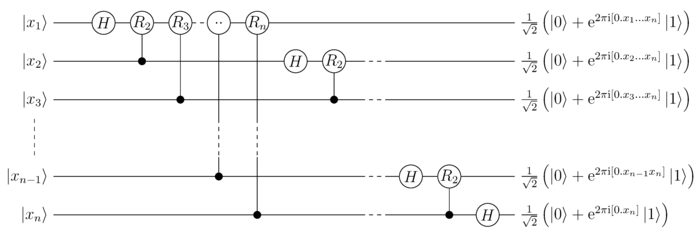
\includegraphics[width=1\textwidth]{images/qft.png}
\label{qft}
\caption{Circuit for the first step of QFT}
\end{figure}
\\The number of gates required to perform this operation is $O(n^2)$ as the $k^{th}$ qubit requires $(n-k+1)$ gates. So in all it requires $O(n^2)$ gates to compute the whole QFT. The complete QFT circuit for $n=3$ is shown on the next page. Note that it requires only 7(or 9 if we consider the $SWAP$ gate as 3 $CNOT$ gates) which is in $O(n^2)$.
\\The inverse of $QFT$ i.e. $QFT^{\dagger}$ can be calculated in a similar way as the only difference in the Fourier and inverse Fourier transform of a series is a negative sign in the exponent. So, by just modifying the $R_k$ gates to have a negative in the exponent, we can compute the inverse transform by using the same circuit.
\begin{figure}[t]
\centering
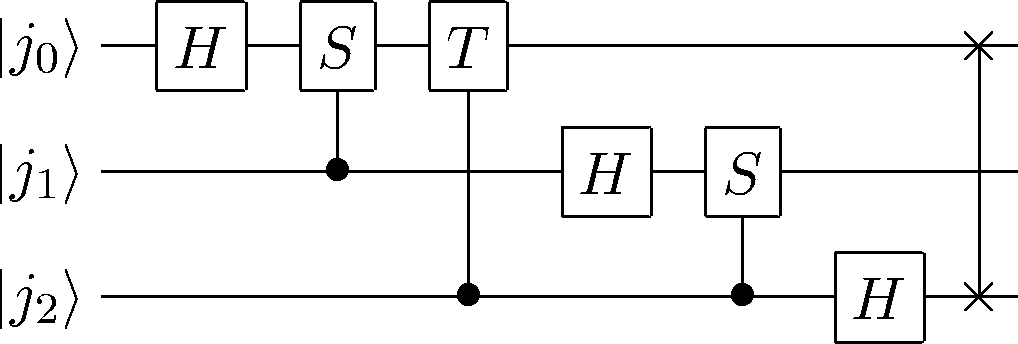
\includegraphics[width=0.75\textwidth]{images/qft3.png}
\label{qft3}
\caption{Circuit for calculating QFT for n=3}
\end{figure}
\newline It turns out that the exponential speed-up for calculating the Fourier Transform has a lot of uses. This allows us to do all the tasks that require the Fourier Transform in exponentially less time.  Most of the algorithms(except for the Quantum Search), including the Shor's Algorithm used to compute the factorisation, that are formed for quantum computing uses this transformation as an essential part.\\

